\section{Sprawdzanie poprawności schematu}
\label{sec:sprawdzanie_poprawnosci_schematu}

Dla każdego poziomu wymagania zapisane są w SO \texttt{Level}, który opisuje,
jakiego rodzaju wymagany jest tranzystor,
między jakimi węzłami powinien się znajdować,
a także jakie są wymagane wymiary bramki.
Przykładowe wymagania dla poziomu 1 przedstawiono na rys.~\ref{fig:level1_requirements}.

\begin{figure}[h]
    \centering
    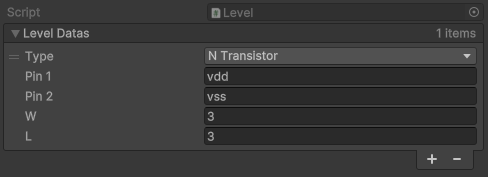
\includegraphics[width=.9\textwidth]{chapters/chapter4/rys/level}
    \caption[Przykładowe wymagania dla poziomu 1.]
    {Przykładowe wymagania dla poziomu 1, źródło: opracowanie własne.}
    \label{fig:level1_requirements}
\end{figure}

Za sprawdzanie poprawności schematu odpowiada komponent \texttt{CheckerManager}, dziedziczący po \texttt{MonoSingleton}.
Zadaniem tego komponentu jest wywołanie komponentu walidującego narysowany schemat,
a następnie porównanie wyników z wymaganiami poziomu.
Na tej podstawie decyduje, czy schemat jest poprawny, czy też nie
i wywołuje okno wyników, które informuje użytkownika o rezultacie.

\subsection{Walidacja schematu}
\label{subsec:walidacja_schematu}

Walidacją schematu zajmuje się komponent \texttt{TopographyValidator}.
Po wywołaniu startu walidacji przez \texttt{CheckerManager},
w pierwszej kolejności wyszukiwane są oznaczenia węzłów, $V_{SS}$ i $V_{DD}$.
Są one punktami zaczepienia dla schematu, a ich brak oznacza błąd.
Gdy znaleziono oba węzły, pobierana jest komórka, jaka znajduje się pod węzłem $V_{DD}$,
przy wykorzystaniu \texttt{Physics.Raycast}.
Komórka ta pełni funkcję punktu startowego w algorytmie znajdywania połączeń.\\
\indent Przed połączeniami, w pierwszej kolejności znajdywane są wszystkie tranzystory na schemacie.
W tym celu z \texttt{LayersManager} pobierane są wszystkie komórki z warstwy \textit{Poly Crystal}.
